\documentclass{article}
\usepackage[margin=1in]{geometry}
\usepackage{microtype}
\usepackage{setspace}
\usepackage{amsmath}
\usepackage{parskip}
\usepackage{amssymb}
\usepackage{graphicx}

\graphicspath{{../public/}}

\parskip=4ex
\date{}
\author{}

\title{13.1 Vector Fields}

\begin{document}
    \maketitle
    In Figure 1(A), the vectors are air velocity vectors indicating the wind speed and direction at points $ 10m $ above the surface elevation in the San Francisco Bay Area at $ 6:00 $ pm on March 1, 2010. 

    THe largest arrows indicate the greatest wind speeds at the the time occured. At every point in the air, there is a wind velocity vector. This is an example of a velocity vector field. 

    \begin{center}
        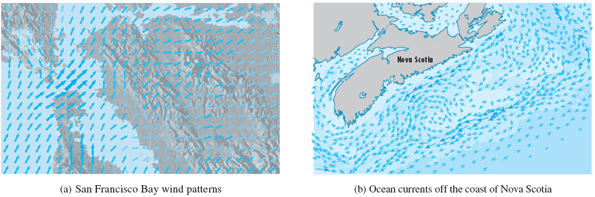
\includegraphics[width=8cm]{13_1_1}
    \end{center}

    Figure 1(B) is another example of a velocity vector field.

    There are other types of vector fields, namely a force field, where each point in a region is associated with a force vector.

    To generalize, a vector field is a function whose domain is a set of points in $ \mathbb{R}^{2} $ or $ \mathbb{R}^{3}  $ and whose range is a set of vectors in $ v_2 $ or $ v_3 $.

    \textbf{Def}\\
    Let $ D $ be a set in $ \mathbb{R}^{2} $ (a plane region). A vector field on $ \mathbb{R}^{2}  $ is a function $ F $ that assigns to each point $ (x,y) $ in $ D $ a two-dimesnional vector $ F(x,y) $.

  Since $ F(x,y) $ is a two-dimensional vector, it can be written in terms of its component functions $ P ~\&~ Q $ as follows
  \[
      F(x,y)=P(x,y)i+Q(x,y)j= <P(x,y), Q(x,y)> 
  \]

  Or, in its shorthanded form,
  \[
      F=Pi+QJ
  \]

  \textbf{Def}\\
  Let $ E $ be a subset of $ \mathbb{R}^{3} $. A vector field on $ \mathbb{R}^{3} $ is a function $ F $ that assigns to each point $ \vec{x,y,z} $ in $ E $ a three-dimensional vector $ F(x,y,z) $.

  Since $ F(x,y, z) $ is a three-dimensional vector, it can be represented in terms of its component functions $ P, Q ~\&~ R $ as
  \[
      F(x,y,z)=P(x,y,z)i+Q(x,y,z)+R(x,y,z)k
  \]

  or, for short,
  \[
      F=Pi+Qj+Rk
  \]
  
 Just like with vector functions, we can define the continuity of vector fields and show that $ F $ is continuous if and only if its component functions $ P, Q, ~\&~ R $ are continuous.

 A point $ (x,y,z) $ is sometimes identified with its position vector $ x=\vec{x,y,z} $ and $ F(x) $ is written in place of $ F(x,y,z) $. Then $ F $ becomes a function that assigns a vector $ F(x) $ to a vector $ x $. 
  
  

\end{document}
